\documentclass[10pt]{beamer}

% theme
\usetheme{PaloAlto}
\usecolortheme{spruce}
\setbeamertemplate{navigation symbols}{}

% packages
\usepackage[utf8]{inputenc}
\usepackage[T1]{fontenc}
\usepackage{graphicx}
\usepackage{caption}
\usepackage{subcaption}
\usepackage{listings}
\usepackage{array}
\usepackage{amsmath}
\usepackage{calc}


% caption settings
\captionsetup{font=scriptsize, skip=2pt}

% listings setting
\lstset{
    captionpos=b,
    label={lst:script},
    basicstyle=\tiny\ttfamily,
    keywordstyle=\color{blue},
    commentstyle=\color{green!60!black},
    numbers=left,
    numberstyle=\tiny\color{gray},
    abovecaptionskip=10pt
}

% cite options
\usepackage[style=verbose,autocite=footnote]{biblatex}
\ExecuteBibliographyOptions{labelnumber}
\AtEveryCitekey{\clearfield{howpublished}}
\addbibresource{../biblio.bib}


% attributes
\title{\textbf{ExaMA WP3 -- Dashboard Performances}}
\author[Tanguy PIERRE]{Tanguy Pierre\\[1cm] \small{Supervisors: V. Chabannes, J. Cladellas}}
\institute{University of Strasbourg}
\date{31st of May}


% **********************  START  **********************
\begin{document}

\frame{\titlepage}


\begin{frame}
    \frametitle{\textbf{Introduction}}

    \begin{itemize}
        \addtolength{\itemsep}{10pt}
        \item Part of the \textit{ExaMA} project from NumPEx 
        \item Benchmarking is for:
        \begin{itemize}
            \item performances comparison
            \item transparency about the evaluation process
            \item references in order to avoid performance decline
            \item data analysis depending on context
        \end{itemize}
    \end{itemize}

    \begin{figure}
        \centering
        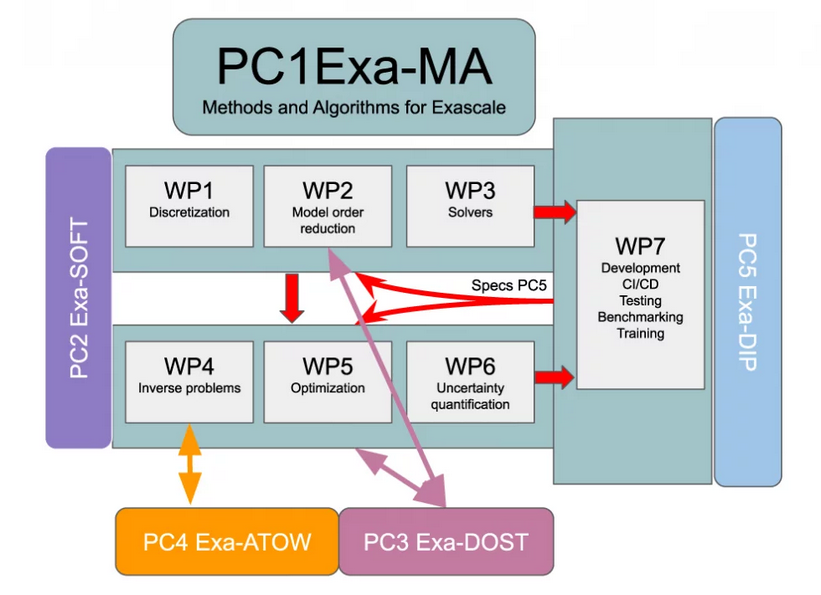
\includegraphics[width=0.6\textwidth]{../illustrations/ExaMa-orga.png}
        \caption{ExaMA organisation}
    \end{figure}
\end{frame}




\begin{frame}
    \frametitle{\textbf{Objectives}}
    \begin{itemize}
        \addtolength{\itemsep}{8pt}
        \item Establish a \textbf{Continuous Integration/Continuous Deployment} workflow. \\
        \item Enhance the \textbf{dashboard presentation} for better visualization of the results. \\
        \item Conducting \textbf{representative tests} is essential to obtain reliable results about the system behaviour. \\
        \item Provide a \textbf{database} for easy access and retrieval of test results. \\
    \end{itemize}

    \begin{figure}
        \centering
        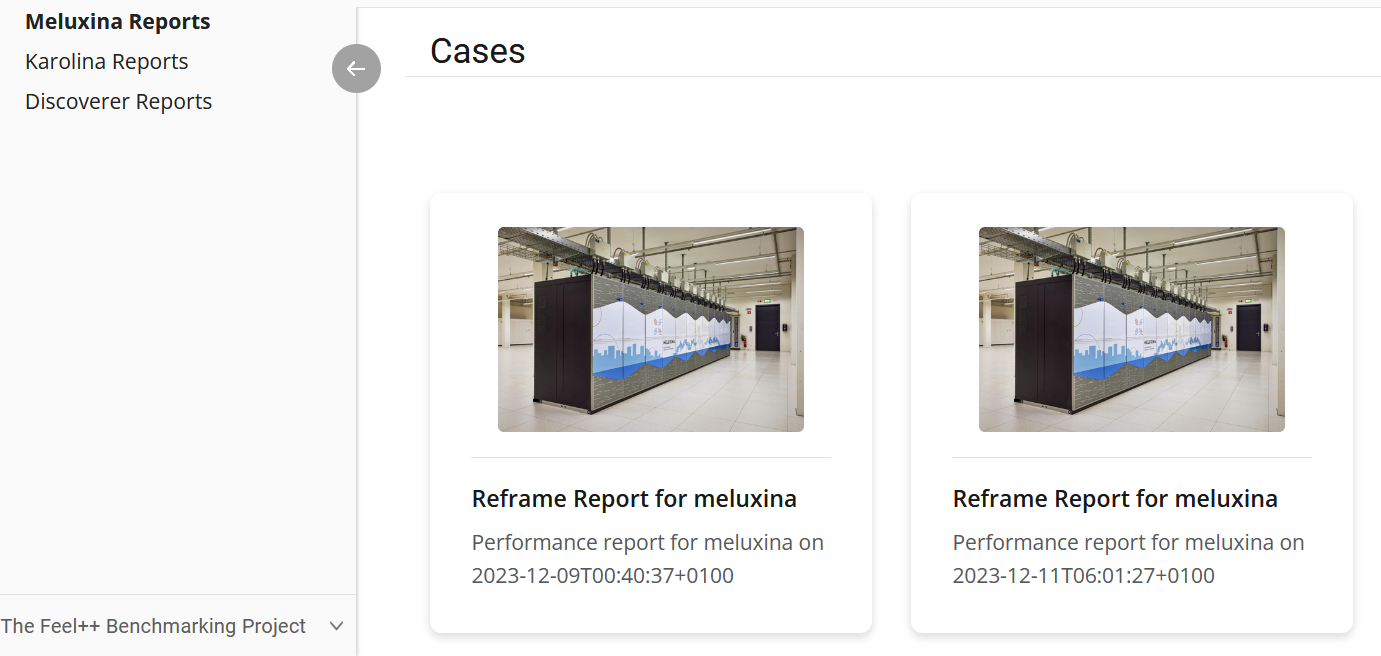
\includegraphics[width=0.6\textwidth]{../illustrations/feelpp-dashboard.png}
        \caption{Feel++ benchmarking platform}
    \end{figure}
\end{frame}

\begin{frame}
    \frametitle{\textbf{Tools}}
    \begin{itemize}
        \addtolength{\itemsep}{7pt}
        \item \textit{ReFrame HPC}, a framework allowing system's complexity abstraction in order to focus only on the algorithm's performance
        \item \textit{Feel++}, a C++ library for Galerkin methods
        \item \textit{Jinja2}, a template engine used for generating the \textit{.adoc}
        \item \textit{Antora}, a documentation site generator \small{(\textit{.adoc} to \textit{.html})}
        \item \textit{Plotly}, the well-known data visualization library
    \end{itemize}

    \begin{figure}
        \centering
        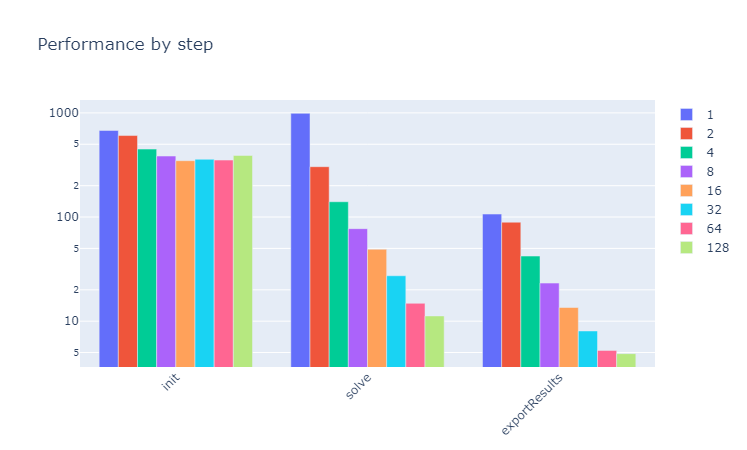
\includegraphics[width=0.6\textwidth]{../illustrations/gaya-graphs/gayaByStep.png}
        \caption{Gaya, Performance by step}
    \end{figure}
\end{frame}


\begin{frame}
    \frametitle{\textbf{Process}}
    \begin{columns}
        \begin{column}{0.5\textwidth}
            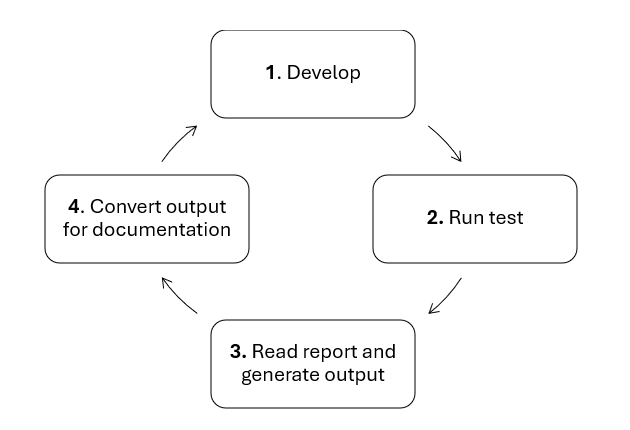
\includegraphics[width=1.1\textwidth]{../illustrations/process.png}
            \captionof{figure}{Gaya, Performance by step}
        \end{column}

        \begin{column}{0.5\textwidth}
            \begin{enumerate}
                \addtolength{\itemsep}{5pt}
                \item Pushing or merging new reports will trigger a new process
                \item Use \textit{ReFrame} for launching multiple tests
                \item \textit{Jinja2} will generate \textit{.adoc} files containing code blocks
                \item \textit{AsciiDoctor} will convert the \textit{.adoc} files into \textit{.html} and Antora will update the documentation site
            \end{enumerate}
        \end{column}
    \end{columns}
\end{frame}

\begin{frame}[fragile]
    \frametitle{\textbf{Process}}
    Here follows the script which controls the launch of the process:
    \vspace{0.5cm}

\begin{lstlisting}[language=bash,caption={Script for process launching}]
rm -rf ~/feelppdb
rm -rf ./build/reframe/output/ ./build/reframe/stage/ ./build/reframe/perflogs

# Variable TO BE SET to the actual HPC
hostname=gaya

current_date=$(date +%Y%m%d)
mkdir -p $(pwd)/docs/modules/${hostname}/pages/reports

export BENCH_CASES_CFG=$(pwd)/src/benchmarking/cases/

# Reframe environment variables
export RFM_CONFIG_FILES=$(pwd)/src/benchmarking/reframe/cluster-config/${hostname}.py
export RFM_REPORT_FILE=$(pwd)/docs/modules/${hostname}/pages/reports/ \
                                            ${hostname}-${current_date}-{sessionid}.json
export RFM_PREFIX=$(pwd)/build/reframe/

reframe -c ./src/feelpp/benchmarking/reframe/regression-tests/heatTest.py \
        -r --system=${hostname} --exec-policy=serial
\end{lstlisting}

\end{frame}

\begin{frame}
    \frametitle{\textbf{Process}}
    \small
    \begin{tabular}{|l|m{8.5cm}|}
        \hline
        \textbf{Line} & \textbf{Description} \\
        \hline
        2-3  & Removing older reports and logs for avoiding unwanted interactions \\
        \hline
        6    & Set up the current machine \\
        \hline
        8    & Get date for reports naming schema \\
        \hline
        9    & Create reports folder if it doesn't already exist \\
        \hline
        11   & Export testcases path \\
        \hline
        14-18   & Export ReFrame environment variables: cluster configuration, report-file with naming schema, output and stage directory\\
        \hline
        20   & Launch Reframe recursevly \textbf{-r} on test defined in the \textit{checkpath} \textbf{-c} with the specified \textit{system}.\\
             & \textbf{--exec-policy=serial} has been set for avoiding some bugs during file access. \\
        \hline
    \end{tabular}
\end{frame}

\begin{frame}
    \frametitle{\textbf{Benchmarking with ReFrame}}
    \framesubtitle{\textbf{Context}}
    \begin{itemize}
        \addtolength{\itemsep}{4pt}
        \item Launching environment description, definition and parametrization
        \item Exact timeline \\
                $\Rightarrow$ decorators for specifying when to launch a particular function
        \item Needs a system configuration file (Python dictionary or \textit{.json} file) \\
        \item Possibility to split the system by partition, node or environment
        \item Reframe offers "sanity functions" to verify test integrity
    \end{itemize}
    \vspace{12pt}
    As we will launch tests with the \texttt{-bind-to core} option from \textit{mpiexec} for maximal efficiency, we are interested in the number of physical cpus on each node,
    which is given by:
    \small{\[ num\_physical\_cpus = num\_sockets * num\_cores\_per\_sockets\]}

\end{frame}

\begin{frame}[fragile]{\textbf{Benchmarking with ReFrame}}
    \framesubtitle{\textbf{Parametrization}}
\begin{lstlisting}[language=python,caption={Task number parametrization, adapted from \footfullcite{CSCS}}]
def parametrizeTaskNumber():
    for part in rt.runtime().system.partitions:
        nbTask = 1
        nbPhysicalCpus = part.processor.num_cpus_per_socket * part.processor.num_sockets
        while nbTask < nbPhysicalCpus:
            yield nbTask
            nbTask <<= 1

        nbNodes = part.devices[0].num_devices
        for i in range(1, nbNodes+1):
            nbTask = i*nbPhysicalCpus
            yield nbTask
\end{lstlisting}


    \begin{itemize}
        \item \texttt{reframe.core.runtime} module to access the host's topology
        \item Parameterization starts with 1 task and increases by power of 2 up to the number of physical CPUs
        \item Then, tasks increase by increments of number of physical CPUs up to this value multiplied by the number of nodes.
    \end{itemize}
\end{frame}

\begin{frame}[fragile]{\textbf{Benchmarking with ReFrame}}
    \framesubtitle{\textbf{Scale performance extraction}}
    \begin{small}
    For extracting performances in the from Feel++ produced files, we work with the \texttt{reframe.utility.sanity} module and regex patterns. \\
    These functions needs the \texttt{@performance\_function} decorator provided by the framework.
    \end{small}
    \begin{tiny}
    \begin{verbatim}
valPatt  = '([0-9e\-\+\.]+)'

@performance_function('s')
def extract_constructor_scale(self, index=1):
    scalePath = os.path.join(self.feelLogPath, 'heat.scalibility.HeatConstructor.data')
    return sn.extractsingle(rf'^{self.num_tasks}[\s]+{self.valPatt}[\s]+{self.valPatt}[\s]+{self.valPatt}[\s] \
                +{self.valPatt}[\s]+{self.valPatt}[\s]+{self.valPatt}[\s]+{self.valPatt}[\s]+{self.valPatt}[\s]+',
                scalePath, index, float)
    \end{verbatim}
    \end{tiny}

    \begin{itemize}
        \item The \textit{self.valPatt}-value at the n-th index of the corresponding pattern will be extracted
        \item The \^{} character guarantees that the expression starts on a new line for avoiding any unintended interaction
        \item Necessary to know the number of values to extract in order to build the pattern \textit{here: 8 values}
    \end{itemize}

\end{frame}

\begin{frame}{\textbf{Benchmarking with ReFrame}}
    \framesubtitle{\textbf{Process extracted data}}
    The \texttt{Report} class is used for extracting the performances. \\
    It will load the ReFrame report and build following dataframes: \\
    \texttt{df\_perf, df\_partialPerf, df\_speedup, df\_partialSpeedup}
    \vspace{10pt}
    \begin{itemize}
        \item The \textit{perf} dataframes are immediately built while reading as they don't need any calculation, they are provided in the report
        \item The \textit{speedup} dataframes are based on a reference value, which is projected to a higher number of tasks. \\
        \item Reference value = performance from the test with the lowest number of tasks.
    \end{itemize}
    \vspace{10pt}
    \textit{Some reports do not include values for partial performances. Therefore, we had to construct two different frames for organizing the data efficiently
            This organization facilitates comparisons between same stage components, especially regarding plotting.}
\end{frame}

\begin{frame}{\textbf{Results}}
    \framesubtitle{\textbf{Case}}
    The following study has been done on case3 from \textit{Thermal Bridges ENISO10122}.
    This is as 3D case representing temperature distribution and heat flows through a wall-balcony junction.

    \begin{figure}
        \centering
        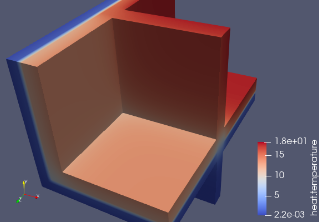
\includegraphics[width=0.3\textwidth]{../illustrations/balcony.png}
        \caption{Case3, Thermal Bridges ENISO10122 \cite*{Feel++}}
    \end{figure}

    \textit{The case is using the case3-bench.cfg configuration file. This file modify some attributes of the case3 located in the Feel++ Heat Toolbox testcases in order to increase the calculation volume: \\
    \begin{itemize}
        \item $ hsize: 0.02 \rightarrow 0.01 $
        \item $ discretization: P1 \rightarrow P2 $
    \end{itemize}}
\end{frame}

\begin{frame}{\textbf{Results}}
    \framesubtitle{\textbf{Single node tests}}
    As Gaya has 128 physical cpus per node, our test has been launched with 1, 2, 4, 8, 16, 32, 64 and 128 tasks.

    \begin{figure}[h]
        \centering
        \begin{subfigure}{0.45\textwidth}
          \centering
          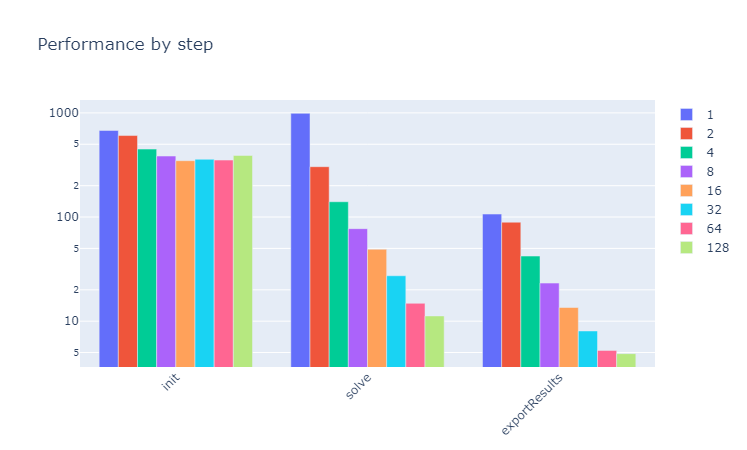
\includegraphics[width=\textwidth]{../illustrations/gaya-graphs/gayaByStep.png}
          \caption{Gaya, Performances by step}
        \end{subfigure}
        \begin{subfigure}{0.45\textwidth}
          \centering
          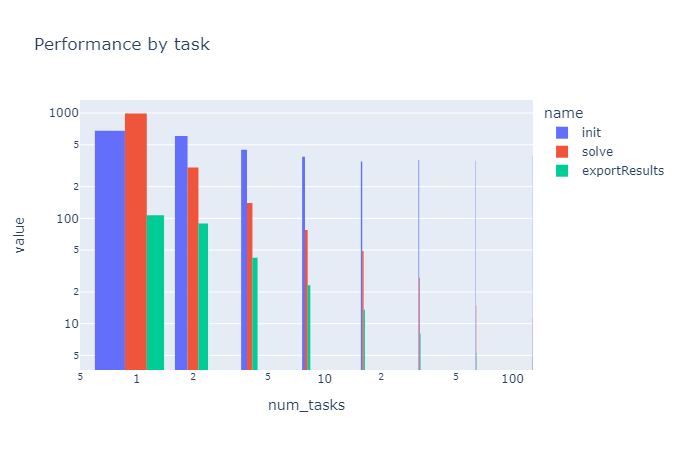
\includegraphics[width=\textwidth]{../illustrations/gaya-graphs/gayaByTask.png}
          \caption{Gaya, Performances by task}
        \end{subfigure}
      \end{figure}

      Both graphics represents the 3 main performances metrics: init, solve and exportResults. \\
      We can easily identify that both \textit{solve}- and \textit{exportResults}-stages do scale well, while it isn't the case for the \textit{init}-phase.
\end{frame}

\begin{frame}{\textbf{Results}}
    \framesubtitle{\textbf{Single node tests}}
    Let's look how the previous 3 main references behave regarding the speedup.

    \begin{figure}[h]
        \centering
        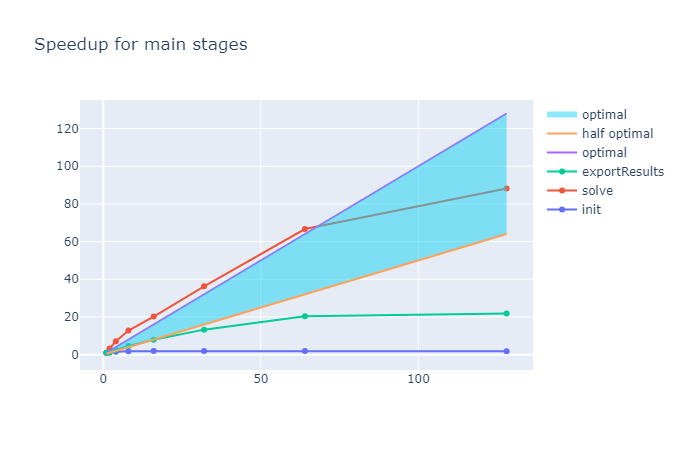
\includegraphics[width=0.8\textwidth]{../illustrations/gaya-graphs/gayaSpeedup.png}
        \vspace{-20pt}
        \caption{Gaya, speedup for main references}
    \end{figure}

    This graph correspond to the previous ones. \\
    As we can see, the \textit{init}-stage doesn't scale at all with increasing number of tasks.
\end{frame}


\begin{frame}{\textbf{Results}}
    \framesubtitle{\textbf{Single node tests}}
    \begin{figure}[h]
        \centering
        \begin{subfigure}{0.49\textwidth}
          \centering
          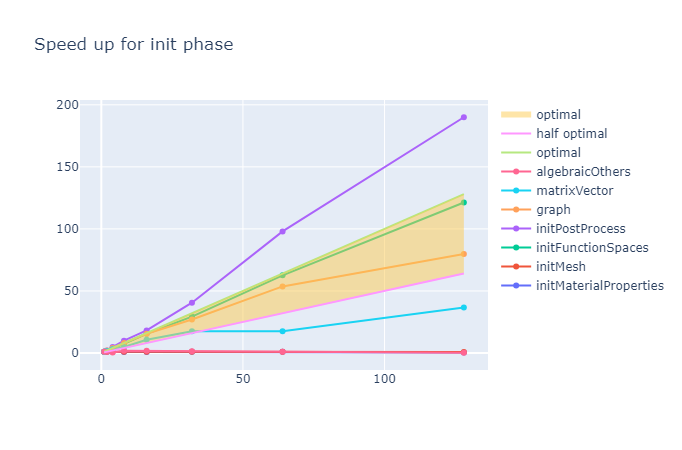
\includegraphics[width=\textwidth]{../illustrations/gaya-graphs/gayaInit.png}
          \caption{Gaya, Performances by step}
        \end{subfigure}
        \begin{subfigure}{0.49\textwidth}
          \centering
          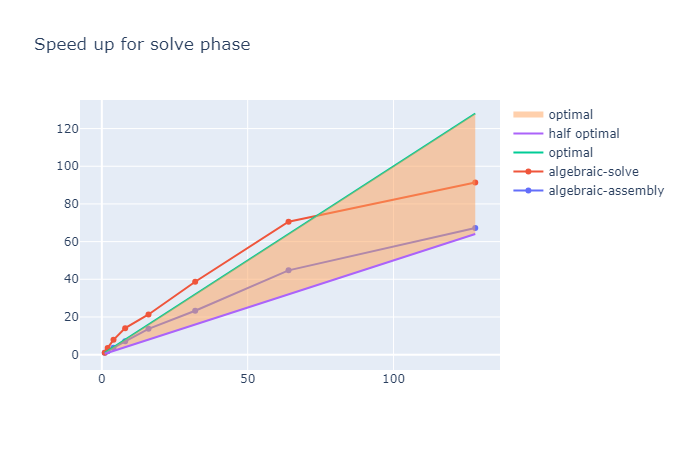
\includegraphics[width=\textwidth]{../illustrations/gaya-graphs/gayaSolve.png}
          \caption{Gaya, Performances by task}
        \end{subfigure}
      \end{figure}

      \begin{itemize}
        \item Figure \textbf{(a)} shows the behaviour of every partial reference obtained through Feel++. \\
                $ \Rightarrow $ \textit{initMesh, initFunctionSpaces and algebraicOthers} jobs run in sequential \\
        \item In contrast, we see in figure \textbf{(b)} that every part of the \textit{solve}-stage scale well. This will of course conduct to great performance for the whole stage.
      \end{itemize}
\end{frame}


\begin{frame}[fragile]
    \frametitle{\textbf{Results}}
    \framesubtitle{\textbf{Multiple nodes tests}}
    Results for multi-node testing are not available yet, since a bug occurs every time a test is launched for number of tasks requiring more than 1 node. \\
    Here are a few lines about this bug: \\

\begin{scriptsize}
\begin{verbatim}
terminate called after throwing an instance of
                'boost::wrapexcept<boost::mpi::exception>'
what():  MPI_Test: MPI_ERR_TRUNCATE: message truncated
*** Aborted at 1716774707 (unix time) try "date -d @1716774707"
                                    if you are using GNU date ***
terminate called after throwing an instance of
                'boost::wrapexcept<boost::mpi::exception>'
*** SIGABRT (@0x10fa00158edd) received by PID 1412829 (TID 0x7fc557cab000)
                                        from PID 1412829; stack trace: ***
\end{verbatim}
\end{scriptsize}

    \textit{Feel++ works with the \textit{Boost.MPI} library, but something doesn't occur well regarding the communication between processors. \\
            The dev-team is already working on it.}
\end{frame}

\begin{frame}{\textbf{Bibliography}}
    \nocite{*}
    \printbibliography[heading=none]
\end{frame}

\end{document}